\documentclass[times, utf8, zavrsni]{fer}
\usepackage{booktabs}
\usepackage{graphicx}
\usepackage{amsmath}
\usepackage{physics}
\usepackage{algorithm}
\usepackage{algorithmic}

\graphicspath{ {./images/} }

\begin{document}

% TODO: Navedite broj rada.
\thesisnumber{000}
\title{Genetski algoritmi inspirirani kvantnom mehanikom}
\author{Juraj Fulir}
\maketitle

% Ispis stranice s napomenom o umetanju izvornika rada. Uklonite naredbu \izvornik ako želite izbaciti tu stranicu.
\izvornik

% Dodavanje zahvale ili prazne stranice. Ako ne želite dodati zahvalu, naredbu ostavite radi prazne stranice.
\zahvala{}

\tableofcontents

\chapter{Uvod}
Svijet koji svakodnevno iskušavamo djeluje nam deterministički.
Dugo vremena fizičari su mislili jednako, sve do početka 19. stoljeća kada su u središte pažnje svijeta fizike došli do tada neobjašnjivi fenomeni.  ............
Primjenom qBita, teoretski je moguće ostvariti značajna ubrzanja nekih NP problema kvantnim algoritama (Shor-ov algoritam faktorizacije cijelih brojeva, Grover-ov algoritam pretrage nesortiranih polja, ...).
Jedan primjer primjene qBita je kvantni registar kao spremnik podataka, kojim se opisuje značaj superpozicije:

\begin{quote}
Pomoću 1 klasičnog registra velićine n bitova moguće je pohraniti 1 od mogućih $2^n$ vrijednosti.

Pomoću 1 kvantnog registra velićine n qBita moguće je pohraniti $2^n$ od mogućih $2^n$ vrijednosti, odnosno sve vrijednosti od jednom.
\end{quote}

\section{Povijest kvantnih algoritama i procesora}
\subsection{Algoritmi}
\subsection{Računala}
\section{Trenutno stanje u svijetu}
Računala (IBM)


\chapter{Kvantni bit (qbit)}
Kvantni bit je najmanja jedinica podatka u kvantnim računalima. Fizički je to zapravo sićušna čestica sa svojstvom superpozicije, jedne od temeljnih fizikalnih pojava u "kvantnom svijetu" čiju ćemo primjenu objasniti u nastavku.

\section{Princip rada}
\paragraph{}
Klasični bit pronalazimo u jednom od dva klasična stanja. Jednom postavljeno stanje se pamti i uvijek ga u njemu možemo pronaći. Njima gradimo binarni brojevni sustav pomoću kojeg zapisujemo podatke na računalu.

\paragraph{}
Kvantni bit ne pamti jedno klasično stanje već se on istovremeno nalazi u više različitih klasičnih stanja. To se svojstvo naziva superpozicija. Fizički gledano kvantni bit je čestica kojoj je pridružen kvantizirani spin. Spin je kvantizirana inačica kutne količine gibanja rotirajućeg tijela.

\paragraph{}
Kvantno stanje jednog qubita opisano je vektorom njegovog spina. Kvantno stanje opisuje vjerojatnost pronalaženja qbita u svakom od klasičnih stanja. Konkretno stanje dobivamo mjerenjem qbita kojim se uništava njegovo svojstvo superpozicije te dobivamo česticu u jednom stanju koju možemo koristiti poput klasičnog bita.

\begin{center}
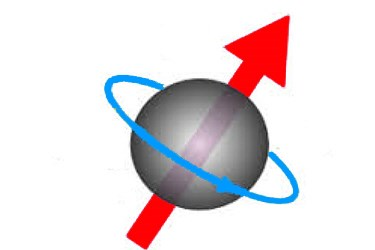
\includegraphics[width=55mm, height=40mm]{spin}
\captionof{figure}{Vjerojatnost pronalaženja qbita u određenom stanju opisana je njegovim kvantnim stanjem (spinom).}
\end{center}

\paragraph{}
Sustavi s kvantnim bitovima mogu biti definirani za proizvoljan brojevni sustav, no kako su današnja računala bazirana na binarnom brojevnom sustavu zanima nas definicija qbita s 2 stanja.

\subsection{Blochova shema}
\paragraph{}
Stanje qbita prikazujemo Blochovom shemom. Jedno kvantno stanje prikazujemo kao vektor iz središta sfere na njezinu površinu. Stanja u kojima možemo pronaći qbit prikazujemo polovima sfere koje definiramo sjecištima sfere i z-osi.

\begin{center}
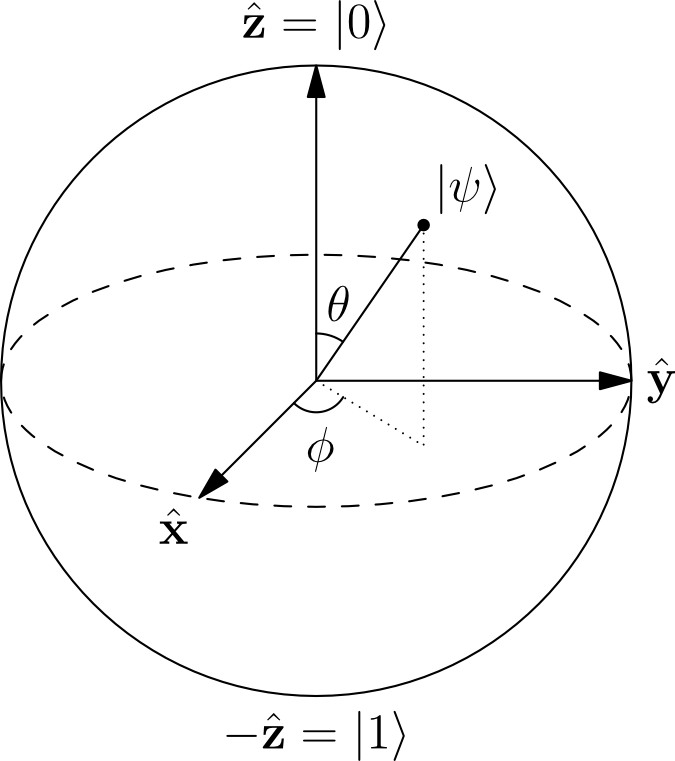
\includegraphics[width=60mm, height=65mm]{bloch}
\captionof{figure}{Blochova sfera}
\end{center}

\paragraph{}
Na slici vidimo jedno kvantno stanje opisano vektorom. Matematički ga možemo opisati kao linearnu kombinaciju dvaju klasičnih stanja:

\begin{align}
\ket{\psi} &= \alpha\ket{0} + \beta\ket{1} \label{eq:psi_orig}
\end{align}

\paragraph{}
Iz Blochove sfere popunjavamo konstante iz \eqref{eq:psi_orig}:

\begin{align}
\ket{\psi} &= \cos(\frac{\theta}{2})\ket{0} + e^{i\phi}\sin(\frac{\theta}{2})\ket{1} \nonumber \\
&= \cos(\frac{\theta}{2})\ket{0} + (cos(\phi)+i\sin(\phi))\sin(\frac{\theta}{2})\ket{1} \label{eq:psi_orig_full}
\end{align}

\paragraph{}
Vrijednosti $\alpha$ i $\beta$ predstavljaju vjerojatnosne amplitude pronalaženja qbita u stanju $\ket{0}$ i $\ket{1}$ respektivno, za koje vrijedi

\begin{equation} \label{eq:prob_norm}
|\alpha|^2 + |\beta|^2 = 1
\end{equation}

\paragraph{}
Iz vjerojatnosnih amplituda računamo vjerojatnosti pronalaženja qbita u svakom od stanja:

\begin{equation} \label{eq:prob}
\begin{split}
\Pr{\ket{0}} = |\alpha|^2 = \cos^2{\frac{\theta}{2}} \\ 
\Pr{\ket{1}} = |\beta|^2 = \sin^2{\frac{\theta}{2}}
\end{split}
\end{equation}

\paragraph{}
Kvantno stanje kraće možemo napisati u obliku vektora:

\begin{equation} \nonumber
\ket{\psi} =
\begin{pmatrix}
\alpha \\ \beta
\end{pmatrix}
\end{equation}

\subsection{Aproksimacija kvantnog stanja}
\paragraph{}
Kvantno stanje prikazano na Blochovoj sferi opisano je u 3 dimenzije. Kako su operacije nad 3 dimenzije računski zahtjevne želimo pojednostaviti model kvantnog stanja. 
Ako pogledamo kvantno stanje opisano formulom \eqref{eq:psi_orig_full} vidimo da $\alpha$ ovisi samo o kutu $\theta$. Kombinacijom formula \eqref{eq:psi_orig_full} i \eqref{eq:prob_norm} zaključujemo kako $\beta$ ovisi isključivo o $\alpha$:

\begin{align*}
\alpha = \cos(\frac{\theta}{2})
\end{align*}
\begin{align*}
|\alpha|^2 + |\beta|^2 &= 1 \\
|\beta|^2 &= 1 - |\alpha|^2 = 1 - \cos^2(\frac{\theta}{2}) = \sin^2(\frac{\theta}{2})
\end{align*}

\paragraph{}
Zaključujemo da je kut $\phi$ suvišan. To možemo vidjeti i na samoj Blochovoj sferi.
Za fiksni kut $\theta$ mijenjanjem kuta $\phi$ rotiramo vektor oko z-osi i ne približavamo se niti jednom polu sfere.

\paragraph{}
Dobivamo sljedeću reprezentaciju kvantnog stanja qbita:

%%%%%%%%%%%%%%%%%
SLIKA 2D

\begin{equation}
\ket{\psi} = \cos(\frac{\theta}{2})\ket{0} + \sin(\frac{\theta}{2})\ket{1}
\end{equation}

\section{Kvantni registar}
Kvantni registar, poput klasičnog registra, pohranjuje niz qbita te omogućuje ne-destruktivno čitanje i zapisivanje istih.

\begin{align*}
\begin{bmatrix}
q_1 & q_2 & q_3 & \cdots & q_i & \cdots & q_n
\end{bmatrix}
\end{align*}

Simulacija kvantnog registra je klasični registar koji pohranjuje vjerojatnosti qbita:

\begin{align*}
\begin{bmatrix}
\alpha_1 & \alpha_2 & \alpha_3 & \cdots & \alpha_i & \cdots & \alpha_n \\
\beta_1 & \beta_2 & \beta_3 & \cdots & \beta_i & \cdots & \beta_n
\end{bmatrix}
\end{align*}

Nadalje moženo dodatno pojednostaviti, u klasični registar pohranjiujemo samo kuteve qbita:
\begin{align*}
\begin{bmatrix}
\theta_1 & \theta_2 & \theta_3 & \cdots & \theta_i & \cdots & \theta_n \\
\end{bmatrix}
\end{align*}



\chapter{Genetski algoritam inspiriran kvantnom mehanikom}
\section{Klasični genetski algoritam (CGA)}
\subsection{Djelovi}
Klasični genetski algoritam zahtjeva nekoliko osnovnih dijelova:
\begin{itemize}
\item Genotip 
\item Operator križanja 
\item Operator mutacije
\item Evaluator 
\end{itemize}

\subsection{Pseudokod}
U ovom primjeru gledamo pseudokod turnirskog algoritma s konstantnom veličinom populacije (SteadyStateTournament).

\begin{algorithm}
\caption{Klasični genetski algoritam (CGA)}
\label{algo:cga}
\begin{algorithmic}
\STATE{p = $InicijalizirajPopulaciju()$}
\STATE{$EvaluirajPopulaciju(p)$}
\STATE{best = $DohvatiNajboljeg(p)$}
\WHILE{$best.fitness.isWorseThan(expectedFitness)$}
\STATE{}
\ENDWHILE
\RETURN best
\end{algorithmic}
\end{algorithm}

\section{Genetski algoritam inspiriran kvantnom mehanikom}
\subsection{Djelovi}
Genetski algoritam inspiriran kvantnom mehanikom uz svoje specifične operatore sadrži i dijelove slične onima iz CGA:
\begin{itemize}
\item Kvantni genotip (kvantni registar)
\item Kvantni operator križanja 
\item Kvantni operator mutacije
\item Operator kvantnih rotacijskih vrata
\item Evaluator
\end{itemize}
\subsection{Pseudokod}
\subsection{Rad algoritma}
\subsection{Implementacijski detalji}


\chapter{Primjena}

\section{Traženje globalnog minimuma funkcije (FunctionMin)}
\subsection{Opis problema}
Zadane su netricijalne funkcije u 3 dimenzije kojima je potrebno pronaći točku minimuma.
Zadane funkcije:
\begin{itemize}
\item Kvadratna
\item Schaffer-ova F6 funkcija
\item Griewangk
\item Ackley
\item Rastrigin
\item Rosenbrock
\item Schaffer-ova F6 funkcija
\end{itemize}

\subsection{Rezultat}

\section{Knapsack problem}
\subsection{Opis problema}
Zadana je nosivost torbe (knapsack) i popis stvari i njima pripadnih težina.
Potrebno je pronaći najbolju kombinaciju stvari uz uvijet da je zadovoljena nosivost torbe.

\subsection{Rezultat}

\section{Regresija neuronske mreže}
\subsection{Opis problema}
Za zadane ulaz/izlaz podatke potrebno je pronaći težine veza neuronske mreže (učenje neuronske mreže).

\subsection{Rezultat}

\section{COCO}
\subsection{Opis problema}
Usporedba s ostalim optimizacijskim algoritmima

\subsection{Rezultat}



\chapter{Moguća nadogradnja}
\section{Paralelizacija}
Stvaranjem više nezavisnih populacija jedinki te povremenom razmjenom najboljih jedinki između populacija poboljšava se rad algoritma.

\section{Podržavanje više-genotipskih jedinki}
Trenutno je ostvarena podrška jedinki s jednim genotipom. Podršku više genotipa moguće je ostvariti izmjenom 'prilagodnika' unutar algoritma te prikladnim zastavicama za odabir genotipa koji će poprimati vrijednosti kvantnog registra.

\chapter{Zaključak}
Zaključak.

\bibliography{literatura}
\bibliographystyle{fer}

\begin{sazetak}
Cilj rada je objasniti koncept pohrane i manipulacije podacima na kvantnim računalima, mogućnost primjene na genetske algoritme na klasičnim računalima te proširenje ECF-a dotičnim algoritmom. Algoritam je primjenjen na 3 različita problema (traženje minimuma, knapsack, regresija neuronske mreže). Rezultati ukazuju na ...

\kljucnerijeci{genetski algoritam, kvantna mehanika, qbit, knapsack, neuronska mreža.}
\end{sazetak}

% TODO: Navedite naslov na engleskom jeziku.
\engtitle{Genetic algorithm inspired by quantum mechanics}
\begin{abstract}
ENGLISH.

\keywords{genetic algorithm, quantum mechanics, qbit, knapsack, neural network.}
\end{abstract}

\end{document}
